\documentclass{article}

% Bibliography
\usepackage{natbib}
\bibpunct{(}{)}{;}{a}{}{;}

% Use 'It was found that A is B (Name 1234)' style
\setcitestyle{authoryear,open={},close={}}

% Affiliations
\usepackage{authblk}
\title{pirouette: the error BEAST2 makes in inferring a phylogeny}
\author[1]{Rich\`el J.C. Bilderbeek}
\author[1]{Giovanni Laudanno}
\author[1]{Rampal S. Etienne}
\affil[1]{Groningen Institute for Evolutionary Life Sciences, University of Groningen, Groningen, The Netherlands}

% Use double spacing
\usepackage{setspace}
\doublespacing

\usepackage{listings}
\usepackage{hyperref}
\usepackage{todonotes}
\usepackage{verbatim}
\usepackage{pgf}
\usepackage{bm}

% Style of listings
% From http://r.789695.n4.nabble.com/How-to-nicely-display-R-code-with-the-LaTeX-package-listings-tp4648110.html
\usepackage{fancyvrb} 
\definecolor{codegreen}{rgb}{0,0.6,0}
\definecolor{codegray}{rgb}{0.5,0.5,0.5}
\definecolor{codepurple}{rgb}{0.58,0,0.82}
\definecolor{backcolor}{rgb}{0.95,0.95,0.92}
\lstdefinestyle{mystyle}{
  language=R,% set programming language
  basicstyle=\ttfamily\small,% basic font style
  commentstyle=\color{gray},% comment style
  % numbers=left,% display line numbers on the left side
  numberstyle=\scriptsize,% use small line numbers
  numbersep=10pt,% space between line numbers and code
  tabsize=2,% sizes of tabs
  showstringspaces=false,% do not replace spaces in strings by a certain character
  captionpos=b,% positioning of the caption below
  breaklines=true,% automatic line breaking
  escapeinside={(*}{*)},% escaping to LaTeX
  fancyvrb=true,% verbatim code is typset by listings
  extendedchars=false,% prohibit extended chars (chars of codes 128--255)
  alsoletter={.<-},% becomes a letter
  alsoother={$},% becomes other
  otherkeywords={!=, ~, $, \&, \%/\%, \%*\%, \%\%, <-, <<-, /},% other keywords
  deletekeywords={c}% remove keywords 
}
\lstset{style=mystyle}

% Adds numbered lines
\usepackage{lineno}
\linenumbers

% Rename 'Abstract' to 'Summary 
\usepackage[english]{babel}
\addto{\captionsenglish}{\renewcommand{\abstractname}{Summary}}

\begin{document}

\maketitle

\begin{abstract}

  \textbf{1. }
    BEAST2 is a popular Bayesian phylogenetics software tool,
    that takes an alignment and inference model to create a
    posterior of jointly-estimated phylogenies and model parameter estimates.
    When a new macro-evolutionary speciation model is developed,
    a good first step is to measure the error BEAST2 makes on known
    phylogeny derived from the new speciation process, 
    with its current set of inference models. \\
  \textbf{2. }
    Here, we present a free, libre and open-source R package, \verb;pirouette;
    that assesses the inference error BEAST2 makes based on a known/true 
    phylogeny. \\
  \textbf{3. }
    We describe \verb;pirouette;'s usage and the biological scientific
    question it can answer, including full examples. \\
  \textbf{4. }
    As \verb;pirouette; is designed to be of high quality and extendable, 
    we conclude by describing the further development of the package. \\
\end{abstract}

{\bf Keywords:} computational biology, evolution, phylogenetics, BEAST2, pirouette, R

%%%%%%%%%%%%%%%%%%%%%%%%%%%%%%%%%%%%%%%%%%%%%%%%%%%%%%%%%%%%%%%%%%%%%%%%%%%%%%%%%%%%%%
\section{Introduction}
%%%%%%%%%%%%%%%%%%%%%%%%%%%%%%%%%%%%%%%%%%%%%%%%%%%%%%%%%%%%%%%%%%%%%%%%%%%%%%%%%%%%%%

Phylogenies are commonly used to explore evolutionary hypotheses.
%Not only can phylogenies show us how species (or other
%evolutionary units) are related to each other, 
%but we can also estimate relevant parameters such as extinction and 
%speciation rates from them.
%There are many phylogenetics tools available to obtain an estimate 
%of the phylogeny of a given set of species. 
%BEAST2 (\cite{bouckaert2014beast}) is one of the most widely used ones.
%It uses a Bayesian statistical framework to estimate 
%the joint posterior distribution of phylogenies and model parameters, 
%from one or more DNA, RNA or amino acid alignments (see figure 1 
%for an overview of the workflow). 

%Here, we present \verb;pirouette;:
%’BEAUti 2, BEAST2 and Tracer for R’, 
%which creates BEAST2 (v.2.4.7) configuration files,
%runs BEAST2, and analyzes its results,
%all from an R function call. This
%will save time, tedious mouse clicking and 
%reduces the chances of errors in such repetitive actions.
%The interface of \verb;pirouette; mimics the tools it
%is based on. This
%familiarity helps both beginner and experienced BEAST2 users 
%to make the step from those tools to \verb;pirouette;.
%\verb;pirouette; enables the creation of a single-script 
%pipeline from sequence alignments to posterior analysis in R. 

%%%%%%%%%%%%%%%%%%%%%%%%%%%%%%%%%%%%%%%%%%%%%%%%%%%%%%%%%%%%%%%%%%%%%%%%%%%%%%%%%%%%%%
\section{Description}
%%%%%%%%%%%%%%%%%%%%%%%%%%%%%%%%%%%%%%%%%%%%%%%%%%%%%%%%%%%%%%%%%%%%%%%%%%%%%%%%%%%%%%

\verb;pirouette; is written in the R programming language (\cite{R}).

\begin{figure}[h]
  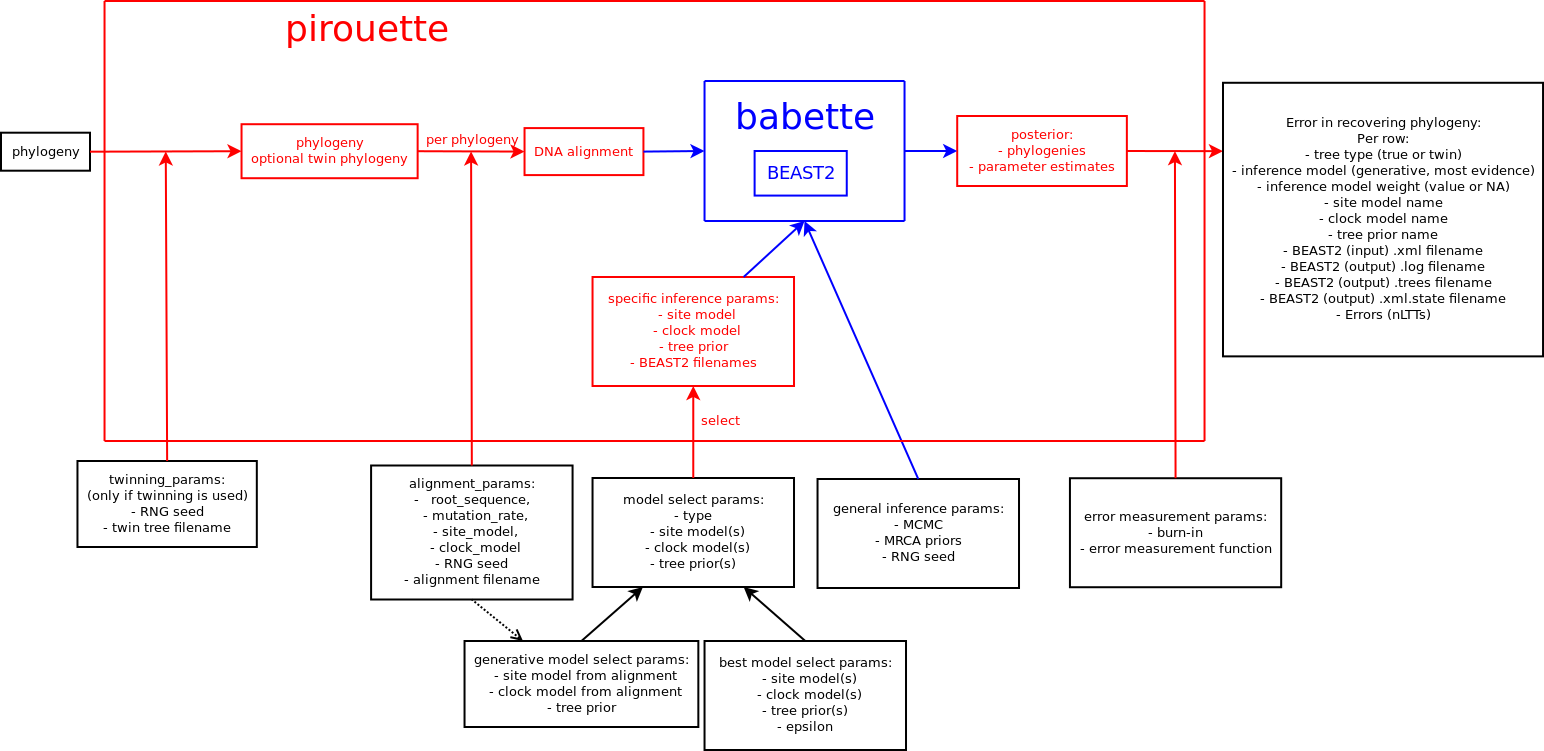
\includegraphics[width=\textwidth]{overview.png}
\end{figure}

and enables the full BEAST2 workflow from a single R function call,
%in a similar way to what subsequent usage of BEAUti, DensiTree and Tracer would produce.
%\verb;pirouette;'s main function is \verb;bbt_run;, which
%configures BEAST2, runs it and parses its output. 
%\verb;bbt_run; needs at least the name of a 
%FASTA file containing a DNA alignment. 
%The default settings for the other arguments of \verb;bbt_run; 
%are identical to BEAUti's and BEAST2's default settings.
%Per alignment, a site model, clock model and tree prior can be chosen.
%Multiple alignments can be used, each with its own (unlinked) site model, 
%clock model and tree prior.

%\verb;pirouette; currently has 108 exported functions to set up  
%a BEAST2 configuration file. 
%\verb;pirouette; can currently handle the majority of BEAUti use cases.
%Because of BEAUti's high number of plugins, 
%\verb;pirouette; uses a software architecture that is designed to be extended.
%Furthermore, \verb;pirouette; has 13 exported functions to run and help run BEAST2.
%One function is used to run BEAST2, another
%one installs BEAST2 to a default location.
%Finally, \verb;pirouette; has 21 exported function to parse the BEAST2 output
%files and analyze the created posterior. \verb;pirouette; gives the
%same ESSes and summary statistics as Tracer. The data is formatted
%such that it can easily be visualized using \verb;ggplot2; (for a trace,
%similar to Tracer) or \verb;phangorn; (\cite{phangorn}) (for 
%the phylogenies in a posterior, similar to DensiTree). 

%Currently, \verb;pirouette; does not contain all functionality 
%in BEAUti, BEAST2 and their many plug-ins, 
%because these tools themselves also change in time.
%\verb;pirouette; currently works only on DNA data,
%because this is the most common use case. 
%Nevertheless, \verb;pirouette; provides the majority of default tree priors and supports the most important command-line arguments of BEAST2, provides
%the core Tracer analysis options, and has the most basic subset of 
%plotting options of DensiTree. Up till now, the \verb;pirouette; features 
%implemented are those requested by users. Further extension of \verb;pirouette; 
%will be based on future user requests.

%%%%%%%%%%%%%%%%%%%%%%%%%%%%%%%%%%%%%%%%%%%%%%%%%%%%%%%%%%%%%%%%%%%%%%%%%%%%%%%%%%%%%%
\section{Installation}
%%%%%%%%%%%%%%%%%%%%%%%%%%%%%%%%%%%%%%%%%%%%%%%%%%%%%%%%%%%%%%%%%%%%%%%%%%%%%%%%%%%%%%

\verb;piouette; can be installed easily from CRAN:

\begin{lstlisting}[language=R, floatplacement=H]
install.packages("piouette")
\end{lstlisting}

For the most up-to-date version, 
one can download and install the package from \verb;pirouette;'s GitHub repository:

\begin{lstlisting}[language=R, floatplacement=H]
usthis::install_github("richelbilderbeek/pirouette")
\end{lstlisting}
To start using \verb;pirouette;, load its functions in the global namespace first:

\begin{lstlisting}[language=R, floatplacement=H]
library(pirouette)
\end{lstlisting}
Because \verb;pirouette; calls BEAST2, BEAST2 must be installed. 
This can be done from within R, using:

\begin{lstlisting}[language=R, floatplacement=H]
install_beast2()
\end{lstlisting}

%%%%%%%%%%%%%%%%%%%%%%%%%%%%%%%%%%%%%%%%%%%%%%%%%%%%%%%%%%%%%%%%%%%%%%%%%%%%%%%%%%%%%%
\section{Usage}
%%%%%%%%%%%%%%%%%%%%%%%%%%%%%%%%%%%%%%%%%%%%%%%%%%%%%%%%%%%%%%%%%%%%%%%%%%%%%%%%%%%%%%

A first research question that \verb;pirouette; answers, is:

What is the error BEAST2 makes from a phylogeny using the same 
speciation model as it was generated by?

Say we have an idealised

\begin{lstlisting}[language=R, floatplacement=H]
phylogeny <- ape::read.tree(text = "((A:4, B:4):1, (C:4, D:4):1);")
\end{lstlisting}


This code will create a (temporary) BEAST2 configuration file,
from the FASTA file with name \verb;anthus_aco.fas; (which
is supplied with the package, from \cite{VanEls2018}), 
using the same default settings as BEAUti, which are, 
among others, a Jukes-Cantor site model, a strict clock, and a Yule birth tree prior.
\verb;pirouette; will then execute BEAST2 using that file, and
parses the output. The returned data structure, named \verb;out;, 
is a list of parameter estimates (called \verb;estimates;), posterior 
phylogenies (called \verb;anthus_aco_trees;, named after
the alignment's name) and MCMC operator performance (\verb;operators;).
An example of using a different site model, clock model 
and tree prior is:

\begin{lstlisting}[language=R, floatplacement=H]
out <- bbt_run(
  fasta_filenames = "anthus_aco.fas",
  site_models = create_hky_site_model(),
  clock_models = create_rln_clock_model(),
  tree_priors = create_bd_tree_prior()
)
\end{lstlisting}
This code uses an HKY site model, a relaxed log-normal clock model and a 
birth-death tree prior, each with their default settings in BEAUti.
Table \ref{tab:functions} shows an overview of all functions to 
create site models, clock models and tree priors.
Note that the arguments' names \verb;site_models;, \verb;clock_models; 
and \verb;tree_priors; are plural, as each of these
can be (a list of) one or more elements. Each of these arguments must 
have the same number of elements, so that each alignment has its
own site model, clock model and tree prior. 
An example of two alignments, each with its own site model, is:

\begin{lstlisting}[language=R, floatplacement=H]
out <- bbt_run(
  fasta_filenames = c(
    "anthus_aco.fas", 
    "anthus_nd2.fas"
  ),
  site_models = list(
    create_tn93_site_model(), 
    create_gtr_site_model()
  )
)
\end{lstlisting}
\verb;pirouette; also uses the same default prior distributions as BEAUti 
for each of the site models, clock models and tree priors. 
For example, by default, a Yule tree prior assumes that the birth rate 
follows a uniform distribution, 
from minus infinity to plus infinity. 
One may prefer a different ddistribution instead. 
Here is an example how to specify an exponential distribution for
the birth rate in a Yule tree prior in \verb;pirouette;:

\begin{lstlisting}[language=R, floatplacement=H]
out <- bbt_run(
  fasta_filenames = "anthus_aco.fas",
  tree_priors = create_yule_tree_prior(
    birth_rate_distr = create_exp_distr()    
  )
)
\end{lstlisting}
In this same example, one may specify
the initial shape parameters of the exponential distribution.
In BEAST2's implementation, an exponential distribution 
has one shape parameter: its mean, which can be set to any
value with \verb;BEAUti;. To set the 
mean value of the exponential distribution to a 
fixed (non-estimated) value, do: 

\begin{lstlisting}[language=R, floatplacement=H]
out <- bbt_run(
  fasta_filenames = "anthus_aco.fas",
  tree_priors = create_yule_tree_prior(
    birth_rate_distr = create_exp_distr(
      mean = create_mean_param(
        value = 1.0, 
        estimate = FALSE
      )
    )    
  )
)
\end{lstlisting}
\verb;pirouette; also supports node dating. Like BEAUti, one
can specify Most Recent Common Ancestor ('MRCA') priors.
An MRCA prior allows to specify taxa having a common ancestor,
including a distribution for the date of that ancestor.
With \verb;pirouette;, this is achieved as follows:

\begin{lstlisting}[language=R, floatplacement=H]
out <- bbt_run(
  fasta_filenames = "anthus_aco.fas",
  mrca_priors = create_mrca_prior(
    taxa_names = sample(get_taxa_names("anthus_aco.fas"), size = 2),
    alignment_id = get_alignment_id("anthus_aco.fas"),
    is_monophyletic = TRUE,
    mrca_distr = create_normal_distr(
      mean = create_mean_param(value = 15.0, estimate = FALSE),
      sigma = create_sigma_param(value = 0.025, estimate = FALSE)
    )
  )
)
\end{lstlisting}
Instead of dating the ancestor of two random taxa, any subset of taxa can be selected,
and multiple sets are allowed.
\verb;pirouette; allows for the same core functionality as Tracer to show the values of the parameter estimates sampled
in the BEAST2 run. This is called the "trace" (hence the name).
The start of the trace, called the "burn-in", is usually discarded, as an MCMC 
algorithm (such as used by BEAST2) first has to converge to
its equilibrium and hence the parameter estimates are not 
representative. By default, Tracer discards the first 10\% of all 
the parameter estimates. 
To remove a 20\% burn-in from all parameter estimates 
in \verb;pirouette;, the following code can be used:

\begin{lstlisting}[language=R, floatplacement=H]
traces <- remove_burn_ins(
  traces = out$estimates, 
  burn_in_fraction = 0.2
)
\end{lstlisting}
Tracer shows the ESSes of each posterior's variables.
These ESSes are important to determine the strength of the
inference. As a rule of thumb, an ESS of 200 is acceptable 
for any parameter estimate.
To calculate the effective sample sizes (of all estimated variables) in \verb;pirouette;:

\begin{lstlisting}[language=R, floatplacement=H]
esses <- calc_esses(
  traces = traces, 
  sample_interval = 1000
)
\end{lstlisting}
Tracer displays multiple summary statistics for each
estimated variable: the mean and its standard error, standard deviation,
variance, median, mode, geometric mean, 95\% highest posterior density interval, 
auto-correlation time and effective sample size. It displays these statistics per
variable. In \verb;pirouette;, these summary statistics are collected for
all estimated parameters at once: 

\begin{lstlisting}[language=R, floatplacement=H]
sum_stats <- calc_summary_stats(
  traces = traces, 
  sample_interval = 1000
)
\end{lstlisting}
\verb;pirouette; allows for the same functionality as DensiTree.
DensiTree displays the phylogenies in a posterior at the same
time scale, drawn one over one another, allowing to see the uncertainty in
topology and branch lengths. 
The posterior phylogenies are stored as \verb;anthus_aco_trees; in the object \verb;out;,
and can be plotted as follows:

\begin{lstlisting}[language=R, floatplacement=H]
plot_densitree(phylos = out$anthus_aco_trees)
\end{lstlisting}
Instead of running the full pipeline, 
\verb;pirouette; also allows to only create a BEAST2 configuration file.
To create a BEAST2 configuration file, with all settings to default, use:

\begin{lstlisting}[language=R, floatplacement=H]
create_beast2_input_file(
  input_filenames = pirouette::get_pirouette_path("anthus_aco.fas"),
  output_filename = "beast2.xml"
)
\end{lstlisting}
This file can then be loaded and edited by BEAUti, 
run by BEAST2, or run by \verb;pirouette;: 

\begin{lstlisting}[language=R, floatplacement=H]
run_beast2(
  input_filename = "beast2.xml",
  output_log_filename = "run.log",
  output_trees_filenames = "posterior.trees",
  output_state_filename = "final.xml.state"
)
\end{lstlisting}
\verb;run_beast2; is a function that only runs BEAST2, 
and does not parse the output files (unlike \verb;bbt_run;). 
In the example above, 
we specify the names of the desired BEAST2 
output files explicitly, and these will be created in the
R working directory, after which they can be inspected 
with other tools, or used to continue a BEAST2 run.
When the names of these files are not specified, 
both \verb;bbt_run; and \verb;run_beast2;
put these files in the default temporary folder (as
obtained from \verb;temp.dir();) to keep
the working directory clean of intermediate files. 

%%%%%%%%%%%%%%%%%%%%%%%%%%%%%%%%%%%%%%%%%%%%%%%%%%%%%%%%%%%%%%%%%%%%%%%%%%%%%%%%%%%%%%
\section{pirouette resources}
%%%%%%%%%%%%%%%%%%%%%%%%%%%%%%%%%%%%%%%%%%%%%%%%%%%%%%%%%%%%%%%%%%%%%%%%%%%%%%%%%%%%%%

\verb;pirouette; is free, libre and open source software available at 
\url{http://github.com/richelbilderbeek/pirouette}
and is licensed under the GNU General Public License v3.0.
\verb;pirouette; uses the Travis CI (\url{https://travis-ci.org})
continuous integration service, which is known to significantly 
increase the number of bugs exposed (\cite{vasilescu2015}) and increases
the speed at which new features are added (\cite{vasilescu2015}).
\verb;pirouette; has a 100\% code coverage, which correlates with 
code quality (\cite{horgan1994,del1995correlation}). 
\verb;pirouette; follows Hadley Wickham's style guide (\cite{style_guide}), 
which improves software quality (\cite{fang2001}).
\verb;pirouette; depends on multiple packages, which are 
\verb;ape; (\cite{APE}), 
\verb;babette; (\cite{babette}),
\verb;ggplot2; (\cite{ggplot2}),
\verb;knitr; (\cite{knitr}),
\verb;mcbette; (\cite{mcbette}),
\verb;phangorn; (\cite{phangorn}),
\verb;rmarkdown; (\cite{rmarkdown}),
\verb;stringr; (\cite{stringr}),
\verb;testit; (\cite{testit}) and 
\verb;usethis; (\cite{usethis}).

\verb;pirouette;'s development takes place on GitHub,
\url{https://github.com/richelbilderbeek/pirouette}, 
which accommodates collaboration (\cite{perez2016ten}) 
and improves transparency (\cite{gorgolewski2016practical}).
\verb;pirouette;'s GitHub facilitates feature requests and 
has guidelines how to do so.

\verb;pirouette;'s documentation is extensive. All functions are documented
in the package's internal documentation. For quick use, 
each exported function shows a minimal example. 
For easy exploration, each exported function's documentation links to related functions.
Additionally, \verb;pirouette; has a vignette that demonstrates extensively how
to use it. There is documentation on the GitHub to get started, 
with a dozen examples of BEAUti screenshots with equivalent \verb;pirouette; code.
Finally, \verb;pirouette; has tutorial videos that can 
be downloaded or viewed on YouTube, \url{https://goo.gl/weKaaU}.

%%%%%%%%%%%%%%%%%%%%%%%%%%%%%%%%%%%%%%%%%%%%%%%%%%%%%%%%%%%%%%%%%%%%%%%%%%%%%%%%%%%%%%
\section{Citation of pirouette}
%%%%%%%%%%%%%%%%%%%%%%%%%%%%%%%%%%%%%%%%%%%%%%%%%%%%%%%%%%%%%%%%%%%%%%%%%%%%%%%%%%%%%%

Scientists using \verb;pirouette; in a published paper can cite this
article, and/or cite the \verb;pirouette; package 
directly. To obtain this citation from within an R script, use:

\begin{lstlisting}[language=R]
> citation("pirouette")
\end{lstlisting}

%%%%%%%%%%%%%%%%%%%%%%%%%%%%%%%%%%%%%%%%%%%%%%%%%%%%%%%%%%%%%%%%%%%%%%%%%%%%%%%%%%%%%%
\section{Acknowledgements}
%%%%%%%%%%%%%%%%%%%%%%%%%%%%%%%%%%%%%%%%%%%%%%%%%%%%%%%%%%%%%%%%%%%%%%%%%%%%%%%%%%%%%%

We would like to thank the Center for Information Technology of the University 
of Groningen for their support and for providing access to the Peregrine 
high performance computing cluster. 
We thank the Netherlands 
Organization for Scientific Research (NWO) for financial support 
through a VICI grant awarded to RSE.

%%%%%%%%%%%%%%%%%%%%%%%%%%%%%%%%%%%%%%%%%%%%%%%%%%%%%%%%%%%%%%%%%%%%%%%%%%%%%%%%%%%%%%
\section{Data Accessibility}
%%%%%%%%%%%%%%%%%%%%%%%%%%%%%%%%%%%%%%%%%%%%%%%%%%%%%%%%%%%%%%%%%%%%%%%%%%%%%%%%%%%%%%

All code is archived at \url{http://github.com/richelbilderbeek/pirouette_article},
with DOI \url{https://doi.org/12.3456/zenodo.1234567}.

%%%%%%%%%%%%%%%%%%%%%%%%%%%%%%%%%%%%%%%%%%%%%%%%%%%%%%%%%%%%%%%%%%%%%%%%%%%%%%%%%%%%%%
\section{Authors' contributions}
%%%%%%%%%%%%%%%%%%%%%%%%%%%%%%%%%%%%%%%%%%%%%%%%%%%%%%%%%%%%%%%%%%%%%%%%%%%%%%%%%%%%%%

RJCB, GL and RSE conceived the idea for the package. 
RJCB created and tested the package, and wrote the first draft of the manuscript.
GL tested the package and contributed substantially to revisions.
RSE contributed to revisions.

%%%%%%%%%%%%%%%%%%%%%%%%%%%%%%%%%%%%%%%%%%%%%%%%%%%%%%%%%%%%%%%%%%%%%%%%%%%%%%%%%%%%%%
% Bibliography
%%%%%%%%%%%%%%%%%%%%%%%%%%%%%%%%%%%%%%%%%%%%%%%%%%%%%%%%%%%%%%%%%%%%%%%%%%%%%%%%%%%%%%
% MEE style
\bibliographystyle{mee}
\bibliography{article}
%%%%%%%%%%%%%%%%%%%%%%%%%%%%%%%%%%%%%%%%%%%%%%%%%%%%%%%%%%%%%%%%%%%%%%%%%%%%%%%%%%%%%%

\end{document}
